\section{Wegematrix}

\begin{frame}{Potenzen einer Adjazenzmatrix}
	Bestimmt die Matrix $A^2$ des folgenden Graphen, wobei $A$ die Adjazenzmatrix bezeichne.
	\begin{figure}[H]
		\centering 
		\begin{tikzpicture}[->,>=stealth,baseline=-5mm]
		\matrix[matrix of math nodes,nodes={draw,circle,minimum size=5mm,inner sep=2pt},row sep=10mm,column sep=10mm,ampersand replacement=\&]
		{
			|(0)| 0 \& |(1)| 1 \& |(2)| 2 \& |(3)| 3 \& \\
		};
		\draw  (0) -- (1);
		\draw (1) -- (2);
		\draw (2) -- (3);
		\path (2) edge [loop below] ();
		\end{tikzpicture}
	\end{figure}
	\pause
	$$ A = \begin{pmatrix}
	0 & 1 & 0 & 0 \\ 0 & 0 & 1 & 0 \\ 0 & 0 & 1 & 1 \\ 0 & 0 & 0 & 0
	\end{pmatrix} \qquad \pause A^2 = \begin{pmatrix}
	0 & 0 & 1 & 0 \\ 0 & 0 & 1 & 1 \\ 0 & 0 & 1 & 1 \\ 0 & 0 & 0 & 0 
	\end{pmatrix} $$ \pause
	$(A^2)_{ij}$ gibt also Auskunft, wieviele Pfade der Länge 2 es von $i$ nach $j$ gibt.\\ \pause 
	$(A^n)_{ij}$ allgemein gibt Auskunft, wieviele Pfade der Länge $n$ es von $i$ nach $j$ gibt. 
\end{frame}

\begin{frame}{Wegematrix}
	\begin{Definition}
		Die Wegematrix $W$ ist definiert als $$W_{ij} = \begin{cases} 0 & (i,j) \notin E^\ast \\ 1 & (i,j) \in E^\ast \end{cases} $$
	\end{Definition}

	\pause
	Dabei ist $E^* = \bigcup_{k=0}^{\infty} E^k$ die \textbf{Erreichbarkeitsrelation}, das ist die reflexiv-transitive Hülle der Kantenrelation $E$.\\
	Es ist $(i,j) \elem E^* \Gdw \text{von $i$ aus ist $j$ \textbf{erreichbar}}.$ \\
	\pause
	Die Wegematrix lässt sich daher folgendermaßen berechnen: 
	$$ W = \sgn\left(\summe{k=0}{n} A^k \right) $$
	
	\pause
	Warum reicht es hier, in der Summe bis $n$ zu gehen?\\ \pause
	Wege mit einer Länge $>n$ enthalten einen Zyklus!
\end{frame}

\begin{frame}{Wegematrix}
	\begin{Beispiel}
		\begin{columns}
			\column{0.4\linewidth}
			\begin{figure}[H]
				\begin{tikzpicture}[->,>=stealth,baseline=-5mm]
				\matrix[matrix of math nodes,nodes={draw,circle,minimum size=5mm,inner sep=2pt},row sep=10mm,column sep=10mm,ampersand replacement=\&]
				{
					|(0)| 0 \& |(1)| 1 \& |(2)| 2 \\
					\& |(3)| 3 \& \\
				};
				\draw  (0) -- (1);
				\draw  (0) -- (3);
				\draw (1) -- (3);
				\draw  (2)  to [bend left] (3);
				\draw  (2) -- (1);
				\draw  (3) to [bend left] (2);
				\draw  (0) to [bend left]  (2);
				\path (2) edge [loop right] ();
				\end{tikzpicture}
			\end{figure}
			\column{0.5\linewidth} \pause
			$$W = \begin{pmatrix}
			1 & 1 & 1 & 1 \\
			0 & 1 & 1 & 1 \\
			0 & 1 & 1 & 1 \\
			0 & 1 & 1 & 1 \\
			\end{pmatrix}$$
		\end{columns}
	\end{Beispiel}
\end{frame}

\begin{frame}{Weiterführendes Material}
	Mehr dazu:
	GBI Übung 10, WS 15/16
\end{frame}

\section{Berechnungsmethoden}

\begin{frame}{Wegematrix-Algorithmus}
	Wie rechnet man das aus? \\
	Naiv:
	\begin{align*}
	&W \leftarrow 0 \\ 
	&\mathbf{for}\ i \gets 0\ \mathbf{to}\ n-1\ \mathbf{do} & \text{// $n$-mal...}  \\
	&\qquad M \gets I \qqquad (I = A^0) \\
	&\qquad\mathbf{for}\ j \gets 1\ \mathbf{to}\ i\ \mathbf{do} & \text{// $i$-mal...} \\
	&\qquad\qquad M \gets M \· A & \text{// $n^2 \· (n + n-1)$ Operationen} \\
	&\qquad\mathbf{od} \\
	&\qquad W \gets W + M & \text{// $n^2$ Operationen} \\
	&\mathbf{od} \\
	&W \gets \sgn(W) &  \text{// $n^2$ Operationen} \\
	\end{align*}
\end{frame}

\begin{frame}{Laufzeit der Berechnung}
	\begin{itemize}[<+->]
		\item Jede Matrix hat $n^2$ Einträge, also ergibt sich für die Summe von $n$ Matrizen $n\cdot n^2=n^3$ Summenoperationen 
		\item  Es gibt $\summe{i=0}{n-1} i = \frac{n(n-1)}{2} $ Matrixmultiplikationen. (Im Algorithmus wird \emph{kein} Speicherplatz für $A^i$ reserviert. Würde bei großen $n$ sehr schnell die Speicherkapazitäten übersteigen.) 
		\item $(B\cdot C)_{ij} = \summe{k=0}{n-1} B_{ik} C_{kj}$, also pro Eintrag einer Matrixmultiplikation, die $n^2$ Einträge hat, $n$ Multiplikationen und $n-1$ Additionen. 
		\item $n^2$ Berechnungen der Signum-Funktion 
	\end{itemize}
	\pause
	Insgesamt also $$ n^2 + n^3 + n^2(n+n-1)\cdot \frac{n(n-1)}{2} = n^5 - \frac{3}{2} n^4 + \frac{3}{2} n^3 + n^2 $$
	Wir betrachten im Allgemeinen nur die führende Ordnung, also $n^5$
\end{frame}

\begin{frame}{Optimierungen}
	Can we do better? \pause
	\bigskip
	
	Betrachten wir nun die Relation $ F = (Id \cup E) $ für eine Kantenmenge $E$. \\  \pause 
	So folgt $$ F^2 = (Id \cup E) \circ (Id \cup E) = Id \cup E \cup E^2 $$ \pause
	Analog : $$ F^4 = (F^2)^2 = (Id\cup E \cup E^2) \circ (Id\cup E\cup E^2) = Id \cup E \cup E^2 \cup E^3 \cup E^4 $$ \pause 
	Also folgt $$ F^{2^m} = \bigcup\limits_{i=0}^{2^m} E^i$$ \\
	Setze $m := \lceil \log_2 n \rceil $.
\end{frame}

\begin{frame}{Optimierungen}
	Can we do better? – Matrixversion \pause
	\bigskip
	
	Betrachten wir nun $ F = (I + A) $ für eine Adjazenzmatrix $A$. \\  \pause 
	So folgt $$ F^2 = (I + A) \· (I + A) = I + A + A^2 $$ \pause
	Analog : $$ F^4 = (F^2)^2 = (I + A + A^2) \· (I + A + A^2) = I + A + A^2 + A^3 + A^4 $$ \pause 
	Also folgt $$ F^{2^m} = \sum\limits_{i=0}^{2^m} A^i$$ \\
	Setze $m := \lceil \log_2 n \rceil $. \pause \impl $W = \sgn\big(F^{2^m}\big)$.
\end{frame}

\begin{frame}
	Der Algorithmus sieht nun also folgendermaßen aus 
	\begin{align*}
		&F \leftarrow A + I & // n^2 \\ 
		&m \leftarrow \lceil \log_2 n \rceil \\
		&\mathbf{for}\ i \leftarrow 1\ \mathbf{to} \ m \ \mathbf{do} & // \lceil \log_2 n \rceil\text{-mal} \\
		&\hspace*{2em} F \leftarrow F \cdot F & // (n+n-1)\cdot n^2 \\
		&\mathbf{od}\\
		& W\leftarrow \sgn(F) 	& // n^2
	\end{align*} \pause
	Wir brauchen also nur noch $n^2 + \lceil \log_2 n \rceil \left( (2n-1)\cdot n^2 \right) +n^2 = \lceil \log_2 n \rceil \cdot 2n^3 + \dots $ Rechenoperationen  \\
\end{frame}

\begin{frame}{Der Warshall-Algorithmus}
	(Noch) schnellere Berechnung der Wegematrix. Laufzeit $O(n^3)$\\
	Mehr dazu in der Vorlesung und im Skript.
	% TODO: Evtl. doch noch anreißen, evtl. zumindest Folie dazu...
\end{frame}

\begin{frame}{Aufgabe 1}
	Gegeben sei folgender Graph $G$ 
	\begin{figure}[H]
		\begin{tikzpicture}[->,>=stealth,baseline=-5mm]
		\matrix[matrix of math nodes,nodes={draw,circle,minimum size=7mm,inner sep=2pt},row sep=20mm,column sep=20mm,ampersand replacement=\&]
		{
			|(0)| 0 \& |(1)| 1 \\
			|(2)| 2 \& |(3)| 3 \\
		};
		\draw (0) -- (1);
		\draw (0) -- (3);
		\draw (1) -- (2);
		\draw (1) -- (3);
		\draw (2) -- (0);
		\path (1) edge [loop right] ();
		\path (2) edge [loop left] ();
		\end{tikzpicture}
	\end{figure}
	Gebt die Adjazenzliste, die Adjazenzmatrix und die Wegematrix zu diesem Graphen an.
\end{frame}

\begin{frame}
	$$ A = 
	\begin{pmatrix} 
	0 & 1 & 0 & 1 \\ 
	0 & 1 & 1 & 1 \\ 
	1 & 0 & 1 & 0 \\ 
	0 & 0 & 0 & 0 
	\end{pmatrix} $$ 
	\pause 
	
	$$W = 
	\begin{pmatrix} 
	1 & 1 & 1 & 1 \\ 
	1 & 1 & 1 & 1 \\ 
	1 & 1 & 1 & 1 \\ 
	0 & 0 & 0 & 1 
	\end{pmatrix}$$
\end{frame}

\begin{frame}{Weitere Graphenprobleme}
	\begin{itemize}[<+->]
		\item Kürzeste Wege
		\item Minimale Spannbäume
		\item (Starke) Zusammenhangskomponenten
		\item Minimale Tour (TSP = Travelling Salesman Problem)
	\end{itemize}
	\thasse{
	\pause
	\begin{figure}[H]
		\centering
		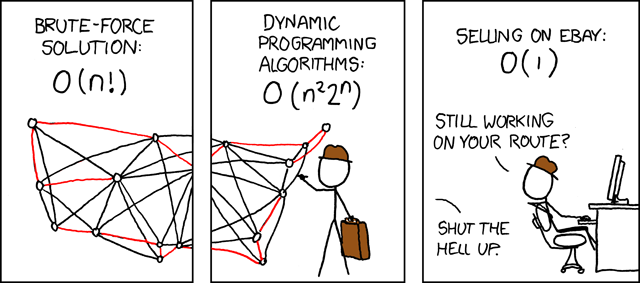
\includegraphics[scale=0.5]{xkcd/tsp_399}
		\caption{ \texttt{\url{http://www.xkcd.com/399}} }
	\end{figure} 	
	}
	

\end{frame}

%\subsection{Warshall-Algorithmus}
%\begin{frame}
%	\only<1>{Schneller geht es mit dem Warshall-Algorithmus!}
%	\only<2>{\begin{align*}
%		&\mathbf{for}\ i\leftarrow 0 \ \mathbf{to} \ n-1 \ \mathbf{do}  \\
%		&\hspace*{2em} \mathbf{for}\ j \leftarrow 0 \ \mathbf{to} \ n-1 \ \mathbf{do} \\
%		& \hspace*{4em} W_{ij} \leftarrow \begin{cases} 1 & i = j \\ A_{ij} & i\neq j \end{cases}  \\
%		&\hspace*{2em} \mathbf{od} \\
%		& \mathbf{od} \\
%		& \mathbf{for}\ k \leftarrow 0 \ \mathbf{to} \ n-1\ \mathbf{do} \\
%		& \hspace*{2em} \mathbf{for}\ i\leftarrow 0 \ \mathbf{to} \ n-1 \ \mathbf{do} \\
%		& \hspace*{4em} \mathbf{for}\ j\leftarrow 0 \ \mathbf{to}\ n-1 \ \mathbf{do} \\
%		& \hspace*{6em} W_{ij} \leftarrow \max\left( W_{ij} , \min(W_{ik},W_{kj}) \right) \\
%		& \hspace*{4em} \mathbf{od}\\
%		& \hspace*{2em} \mathbf{od} \\
%		& \mathbf{od} 	
%		\end{align*}}
%	\only<3>{\begin{align*}
%		&\mathbf{for}\ i\leftarrow 0 \ \mathbf{to} \ n-1 \ \mathbf{do} & // n  \\
%		&\hspace*{2em} \mathbf{for}\ j \leftarrow 0 \ \mathbf{to} \ n-1 \ \mathbf{do} & // n \\
%		& \hspace*{4em} W_{ij} \leftarrow \begin{cases} 1 & i = j \\ A_{ij} & i\neq j \end{cases} & // 1 \\
%		&\hspace*{2em} \mathbf{od} \\
%		& \mathbf{od} \\
%		& \mathbf{for}\ k \leftarrow 0 \ \mathbf{to} \ n-1\ \mathbf{do} & // n \\
%		& \hspace*{2em} \mathbf{for}\ i\leftarrow 0 \ \mathbf{to} \ n-1 \ \mathbf{do} & // n \\
%		& \hspace*{4em} \mathbf{for}\ j\leftarrow 0 \ \mathbf{to}\ n-1 \ \mathbf{do} & // n \\
%		& \hspace*{6em} W_{ij} \leftarrow \max\left( W_{ij} , \min(W_{ik},W_{kj}) \right) & // 1 \\
%		& \hspace*{4em} \mathbf{od}\\
%		& \hspace*{2em} \mathbf{od} \\
%		& \mathbf{od} 	
%		\end{align*}}
%\end{frame}
%
%\begin{frame}
%	\frametitle{Der Warshall-Algorithmus}
%	Da wir hier binäre Werte haben, gilt: $$ \max\left( W_{ij} , \min(W_{ik},W_{kj}) \right) = W_{ij} \vee \left( W_{ik} \wedge W_{kj} \right) $$ \pause 
%	Es ergibt sich insgesamt also eine Laufzeit von $$ n^3+n^2$$ 
%\end{frame}
%
%\begin{frame}
%	\frametitle{Der Warshall-Algorithmus}
%	Was sagt die Matrix $W$ an der Stelle $W_{ij}$ nach dem $k-ten$ Durchlauf im Warshall-Algorithmus aus? \\ \pause
%	Stimmt dieser Algorithmus eigentlich?
%\end{frame}
%
%\begin{frame}
%	\frametitle{Warshall beweisen}
%	\begin{block}{Schleifeninvariante}
%		Für alle $i,j\in \G_n \wedge i\neq j$ gilt : Nach $k$ Durchläufen hat die Matrix den Wert $1$ an der Stelle ($i,j$), genau dann wenn es einen wiederholungsfreien Pfad von $i$ nach $j$ über Knoten in $\G_k$ gibt. Bei $i=j$ steht dort eine $1$. \\
%	\end{block}	
%	
%	\pause
%	Beweis auf Seite 117 im GBI-Skript von Herr Worsch. 
%\end{frame}


%\subsection{Aufgabe 2}
%\begin{frame}
%	\frametitle{Aufgabe 2}
%	Gegeben sei folgende Adjazenzmatrix $$ A = \begin{pmatrix}
%	0 & 1 & 0 & 1 & 1 \\ 0 & 1 & 0 & 1 & 0 \\ 1 & 1 & 0 & 1 & 1 \\ 1 & 1 & 1 & 0 & 1 \\ 0 & 0 & 0 & 0 & 0 
%	\end{pmatrix} $$ 
%	Zeichnen Sie den dazugehörigen Graphen und geben Sie die Initialisierungsmatrix sowie alle Zwischenmatrizen beim Warshall-Algorithmus an. 
%\end{frame}
%
%\subsection{Lösung zu Aufgabe 2}
%\begin{frame}
%	\begin{figure}[H]
%		\begin{tikzpicture}[->,>=stealth,baseline=-5mm]
%		\matrix[matrix of math nodes,nodes={draw,circle,minimum size=9mm,inner sep=2pt},row sep=10mm,column sep=10mm,ampersand replacement=\&]
%		{
%			|(0)| 0 \& \& |(1)| 1 \\
%			\& |(3)| 3 \\
%			|(2)| 2 \& \& |(4)| 4 \\
%		};
%		\draw (0) -- (1);
%		\draw (0) to [bend right] (3);
%		\draw (0) to [bend right] (4) ;
%		\path (1) edge [loop right] ();
%		\draw (1) to [bend right] (3);
%		\draw (2) -- (0);
%		\draw (2) to [bend left] (1);
%		\draw (2) -- (4);
%		\draw (3) to [bend right] (0);
%		\draw (3) to [bend right] (1);
%		\draw (3) -- (2);
%		\draw (3) -- (4);
%		\end{tikzpicture}
%	\end{figure}
%\end{frame}
%
%\begin{frame}
%	$$ W_I = \begin{pmatrix}
%	1 & 1&0&1&1\\0&1&0&1&0\\1&1&1&1&1\\1 & 1 & 1 &1 &1 \\ 0 & 0 & 0 & 0 & 1 
%	\end{pmatrix} $$ \pause
%	$$ W_0 = W_I = W_1 = W_2 $$ \pause
%	$$ W_3 = \begin{pmatrix}
%	1 & 1 & 1 & 1 & 1 \\ 1 & 1 & 1 & 1 & 1 \\ 1 & 1 & 1 & 1 & 1 \\ 1 & 1 & 1 & 1 & 1 \\ 0 & 0 & 0 & 0 & 1 
%	\end{pmatrix} $$ \pause
%	$$ W_4 = W_3 = W$$ 
%\end{frame}